\chapter{Marco teórico}
Aquí va el marco teórico.

\section{Primera sección}
Esta es la primera sección del marco teórico.
	\subsection{Subsección uno}
	Esta es la subsección
	\begin{figure}[htb]
	\centering
	
\includegraphics[scale=0.4]{Img/1.png}
	\caption{Imagen 1}
	\end{figure}
		\subsubsection{SubSubsección uno}
	\begin{figure}[htb]
	\centering
	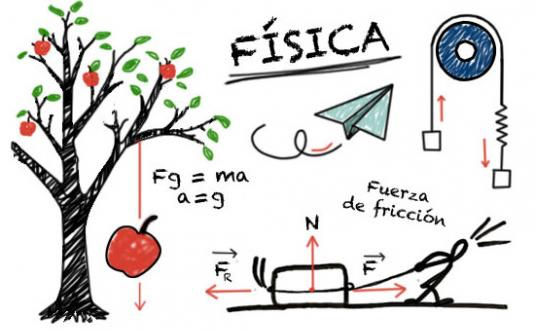
\includegraphics[scale=0.4]{Img/2.png}
	\caption{Imagen 2}
	\end{figure}
		\subsubsection{SubSubsección dos}
	\begin{figure}[htb]
	\centering
	
\includegraphics[scale=0.4]{Img/3.png}
	\caption{Imagen 3}
	\end{figure}
		\subsubsection{Sub-Subsección tres}
	\subsection{Subsecci\'on dos}
	Esta es la subsecci\'on dos

\section{Segunda sección}
Esta es la segunda secci\'on del marco te\'orico.
\begin{table}[htb]
\centering
\caption[Tabla 1]{Esto es un ejemplo de tabla}
\begin{tabular}{|c|c|}
\hline 
casas & mama \\ 
\hline 
tablas & papa \\ 
\hline 
\end{tabular} 
\end{table}
